\documentclass{article}
\usepackage{ijcai11}
\usepackage{lipsum}
\usepackage{mathptmx}
\usepackage[scaled=.90]{helvet}
\usepackage{courier}
\usepackage{latexsym} 
\usepackage{todonotes} 
\usepackage{amsmath} 
\usepackage[dutch]{babel} 

%visuals
\graphicspath{{visuals/}}


\title{Internet of Things code deployment metrics}
\author{Ward Schodts \and Xavier Go\'as Aguililla \\ ward.schodts@student.kuleuven.be \\ xavier.goas@student.kuleuven.be}

\begin{document}

\maketitle

\listoftodos

\begin{abstract}
Wij stellen een simpele vuistregel voor die kan dienen om te beslissen of een
bepaald stuk applicatielogica op een mote kan draaien zonder lokaal energie- of
performantieverlies. 
  
\end{abstract}

\section{Situering \& probleemstelling}

\todo[inline]{explain what WSNs are?}

\subsection{Onderzoeksvraag}

Een typische mote heeft erg beperkte reken- en opslagcapaciteit, wat verhindert
dat er meerdere processen op effici\"ente wijze concurrent kunnen worden
uitgevoerd. In het algemeen gaat men daarom een simpele strategie toepassen voor
dataverwerking, waarbij de mote \'e\'en enkele verantwoordelijkheid heeft, het
zgn. 'sense and send': sensordata wordt op de motes niet bewerkt, maar meteen
doorgestuurd naar de backend voor verdere verwerking, waardoor de rol van de
motes bij het verwerken van de data geminimaliseerd wordt.

Dit is de na\"iefste aanpak die men kan gebruiken, en steunt net op het deel van
mote dat het gulzigst is met energie: de antenne.  De vraag dringt zich op: is
er geen manier om van de weliswaar beperkte rekenkracht van de motes gebruik te
maken om effici\"enter om te springen met de antenne? En is het mogelijk een
simpele, algemene maatstaf te gebruiken om te beslissen of dit in een specifiek
deployment scenario kan of niet?

Energie-effici\"entie is een cruciale factor op alle niveaus bij het
ontwikkelen van wireless sensor networks: een typische mote heeft geen toegang
tot een onbeperkte stroombron en moet het doen met een batterij. Deze batterij
kan in veel scenario's waarin WSNs worden gebruikt ook niet hernieuwd worden, en
dus is de levensduur van de mote ook afhankelijk van hoe zuinig hij omspringt
met energie. Het is dan ook geen wonder dat veel research in het gebied
rechtstreeks wordt be\"invloed door deze kwestie: van de ontwikkeling van
besturingssystemen voor motes over netwerkprotocollen tot studies van
netwerktopologie\"en.

Het ontwikkelen van een eenvoudige metric die een programmeur toelaat om snel en
efficiënt te evalueren of een bepaalde applicatie op een mote kan gedeployed
worden of niet zou interessant zijn voor het ontwikkelen van
energie-effici\"ente IoT-systemen. Bovendien zou daarmee een waardevolle
bijdrage kunnen geleverd worden over het ontwikkelen van IoT-architecturen in
het algemeen.

\subsection{Onderzoeksopgave}

Een eenvoudige vuistregel, die:
\begin{itemize}
\item In de grote meerderheid van de gevallen een juiste beslissing zal maken;
\item eenvoudig te integreren is in de ontwikkelingscyclus;
\item semi-automatisch werkt.
\end{itemize}

\section{Voorgestelde oplossing}
We vertrekken vanuit de veronderstelling dat de ontwikkelaar een stuk
applicatielogica rechtstreeks op de motes wilt deployen. Vanuit deze optiek
maken we abstractie van de low-level details van simulatie e.d., en gebruiken we
in plaats daarvan een eenvoudige vuistregel (\textit{code deployment
metric}. Deze geeft een makkelijke ja/nee-beslissing die zegt of we kunnen
deployen of niet. We defini\"eren een functie $h$ voor deze vuistregel als
volgt:
% \begin{equation}
%   \begin{split}
%     h : x \mapsto \{0, 1\} \\
%     h(x) = signum(transmit(x) - cost(reduce(x)) \\ - cost(transmit(reduce(x))))
%   \end{split}
% \end{equation}

\[
h(x)= 
\begin{cases}
  1, & \text{als } tr(x) - cost(red(x)) - cost(tr(red(x))) > 0  \\
  0, & \text{in alle andere gevallen}
\end{cases}
\]

Waarbij $n$ de grootte van de sensordata in bytes is, en $m$ de verwachte
grootte van de output van de functie compute toegepast op de sensorinput, ook in
bytes.

Wat deze ongelijkheid afweegt is: gegeven een reductie van de sensordata van $n$ naar
$m$ bytes, is de som van de kost van deze reductie op een input van een bepaalde
grootte en de kost van het verzenden van de output van deze reductie kleiner dan
de kost van het verzenden van de originele input?

De aard van deze reductie ligt niet vast. In eerste instantie zouden we kunnen
denken aan een louter computationeel proces dat het aantal over te dragen bytes
reduceert en dan meteen overdraagt. Zo'n voorbeeld is een filter: we sturen een
meting pas door als die verschilt van de vorige verstuurde meting. Maar we
kunnen evengoed de sensordata aggregeren in het geheugen, zodat de transferkost
wanneer een meting binnenkomt nul wordt, behalve als de buffer waarin we data
opslaan vol is.\footnote{Merk ook op dat de kost van het verzenden van gegevens
niet lineair is -- er is geen garantie dat $cost(transfer(x)) +
cost(transfer(y)) = cost(transfer(x + y))$. In een keer $x + y$ bytes versturen
kan dus voordeliger uitkomen dan $x$ en $y$ bytes apart te verzenden.} 
Ook een combinatie van beide is mogelijk: we kunnen bijvoorbeeld de buffer
comprimeren door reeksen identieke metingen samen te nemen (filter +
aggregator). Dit zou theoretisch gezien een grotere winst moeten opleveren.

De aandachtige lezer stelt zich meteen de vraag: hoe kunnen wij de kost van zo'n
reductie in het algemeen schatten, zuiver uitgaand van het programma? 

\todo[inline]{uitweiden}

We laten de programmeur, die zijn programma goed kent, ingrijpen. We nemen als
input niet enkel het gecompileerde programma, maar ook een set parameters. Deze zijn bijvoorbeeld:

\paragraph{Sensoren.} Hoe groot is de sensordata? Hoe vaak komt er sensordata binnen?
\paragraph{Geheugenverbruik.} Worden er gegevens bijgehouden in een buffer? Hoeveel? Hoe vaak wordt er naar die buffer geschreven?
\paragraph{Nauwkeurigheid.} Wat is de gewenste granulariteit van de metingen,
d.w.z. hoe groot mag het interval tussen twee doorgestuurde metingen zijn?
\paragraph{Tijdsinformatie.} Hoe vaak wordt er data verzonden?
\paragraph{Kostfunctie.} Hoeveel kost de reductie aan CPU-tijd?
\paragraph{Reductiegrootte.} Hoe sterk verkleint de reductie het aantal te
verzenden bytes?

\section{Methodologie}

De kwestie is nu om wat we theoretisch uiteen hebben gezet in te vullen met
empirische data: hoe berekenen wij de kost van het verzenden en verwerken van
gegevens concreet? We berekenen het kostenplaatje \textit{atomisch}: we kiezen
bepaalde eenheden voor de drie componenten van het energieverbruik die we kunnen
be\"invloeden:

\begin{itemize}
\item \textbf{storage}: hoeveel kost het om $n$ bytes op te slaan in het RAM of
het EEPROM?
\item \textbf{computation}: hoeveel kosten $n$ seconden CPU-tijd?
\item \textbf{transmission}: hoeveel kost het om $n$ bytes te verzenden; hoeveel
kost het om de antenne aan en uit te zetten?
\end{itemize}

Een eerste reflex is om naar de technische fiche van de motes te grijpen. die
zijn dan wel vrij betrouwbaar, maar geven metingen weer die als het ware in een
vacu\"um zijn gedaan: de kost van het draaien van het OS, van het op laten staan
van de antenne in low power listening modus, enz. worden hierin niet
meegerekend. We zijn daarom experimenteel gaan uitzoeken wat de kost was van elk
van deze types.

\subsection{Meetopstelling en materialen}

Voor onze metingen maakten wij gebruik van de AVR Zigduino. Deze werd
aangesloten op een circuit met spanning 6V en stroom 0.04A.

Voor het meten van het energieverbruik gedurende een bepaalde periode maken we gebruik van het volgende circuit:

\begin{figure}[h]
\centering
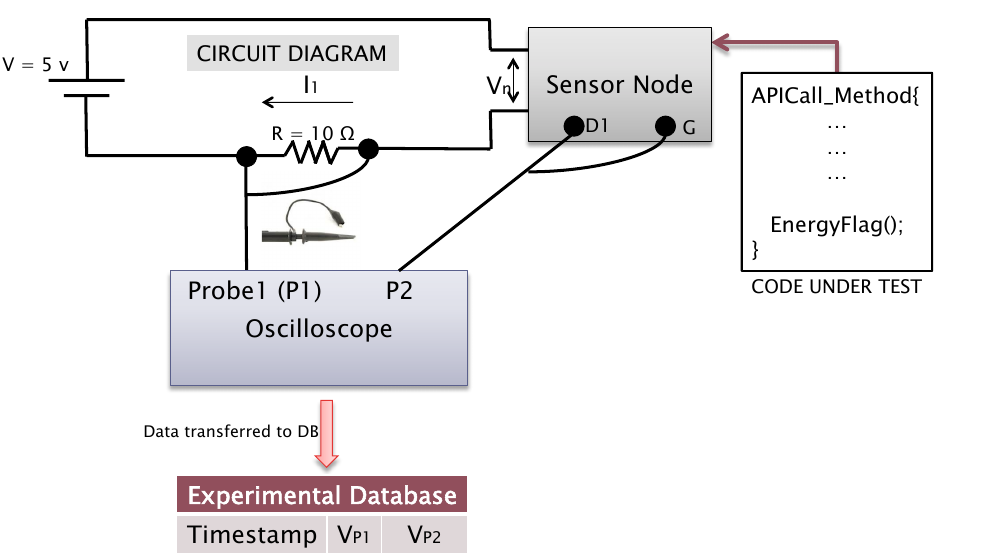
\includegraphics[width=9cm]{meetopstelling}
\caption{De meetopstelling}
\label{fig:meetopstelling}
\end{figure}

De oscilloscoop meet de spanning in het circuit. De weerstand kan aan en uit
worden gezet door de mote door het pin-outsignaal te flippen. Er is enkel stroom
in het circuit verbonden aan de pin-out als het signaal op hoog staat; die
periodes zijn duidelijk af te lezen op de output van oscilloscoop en komen
overeen met de periodes waarin de code waarvan we het energiegebruik willen
kennen wordt uitgevoerd. We kunnen gebruik maken van de wet van Ohm om de
verbruikte stroom in die intervallen te schatten. Daardoor kunnen we met goede
precisie meten hoeveel energie een bepaald stuk code verbruikt.

\subsection{De tool}

\paragraph{Input voor de tool}
De tool is geschreven in Python en volgt een simpel stramien: in de directory
waarin het Contiki-programma staat, moet een parameterbestand in
Python-configuratieformaat worden opgeslagen. Dat zal er ongeveer als volgt
uitzien:

\begin{verbatim}
[sensor]
sensor_data_size = <int n>
sensor_data_frequency = <float f>
[memory]
buffer_used = <bool b>
buffer_size = <int n>
buffer_write_freq = <int n>
[precision]
interval_granularity = <float f>
data_granularity = <float f>
[frequency]
reduction_frequency = <float f>
transmission_frequency = <float f>
reduction_cpu_time = <int n>
[reduction]
from = <int n>
to = <int m>
\end{verbatim}

\paragraph{Parameters schatten.} Sommige van deze parameters liggen niet meteen
voor de hand. Bij deze een aantal manieren die we gebruikt hebben om deze
parameters te schatten:

\subparagraph{Kost van de reductie: CPU-tijd.} Momenteel werken wij aan een
methode om bijna volledig automatisch te bepalen hoeveel CPU-tijd het uitvoeren
van de reductie ongeveer kost. Deze is echter nog niet volledig op punt. Een
andere methode is het gebruik van een fysiek meetapparaat om op een soortgelijke
wijze als bij de energiemetingen te kijken hoe lang het duurt voor de reductie
uitgevoerd is. Dit geeft een harde bovengrens voor de gebruikte CPU-cycli: we
hoeven slechts deze tijd te vermenigvuldigen met de klokfrequentie van de
CPU. Bij de Zigduino is dit 16MHz.

\subparagraph{Reductiegrootte.} De reductiegrootte is vaak
niet op het eerste zicht in te schatten. Een voorbeeld: neem dat wij een
temperatuur- en vochtigheidssensor hebben, en we willen op elk mogelijk moment
weten of het aangenaam of niet aangenaam is waar de mote staat, en we steken dit
in juist één byte. Dan hebben wij de temperatuur (bijv. twee bytes) en de
vochtigheidsgraad (bijv. ook twee bytes) gereduceerd naar \'e\'en byte. Dit
kunnen we zeer gemakkelijk uitwerken.

Maar als we bijvoorbeeld een filter toepassen op onze gegevens, en enkel data
verzenden wanneer we een significant ander resultaat hebben dan bij de vorige
meting, dan wordt de situatie complexer: dan hangt de reductiegrootte af van
bv. hoeveel we willen dat het resultaat van de vorige metingen verschilt voor we
versturen, hoe vaak de temperatuur en vochtigheidsgraad schommelen op die plek
(wat op zich weer afhangt van allerlei factoren in de omgeving), enzoverder.

In zo'n situatie is het aangewezen om een slimmere schatting te maken. Een optie
is om via \textit{sense and send} een steekproef te doen van de temperatuur en
vochtigheidsgraad en hieruit af te leiden hoe sterk de temperatuur en
vochtigheidsgraad zullen oscilleren.

Een andere mogelijkheid is het afschatten van de reductiegrootte door de
worst-case reductiegrootte te bekijken.

\subparagraph{Tijdsinformatie.} Merk op dat in het zonet vermelde geval ook de
tijdsinformatie op een gelijkaardige manier moet worden afgeleid. De frequentie
waarop sensordata binnenkomt kan men makkelijk vinden, de frequentie waarmee die
data verzonden wordt soms niet. 

\subparagraph{Geheugenverbruik, sensoren, precisie.} Deze liggen geheel in de
hand van de programmeur; er zijn echter een aantal edge cases. 

\subsection{Een concreet stappenplan voor deployers}
We mikken erop om het beslissingsproces zo goed mogelijk te integreren in
de ontwikkelingsomgeving van Contiki. Men werkt daar voornamelijk met
\texttt{make}-bestanden. Een typische workflow zou er als volgt moeten uitzien.

\begin{enumerate}
\item Schrijf het gewenste programma.
\item Maak een parameterbestand aan. Schat de parameters zoals hierboven
aangegeven en verwerk ze hierin.
\item Voer het commando \texttt{make eval-metric} uit. Dit 
\end{enumerate}

\subsection{Een voorbeeldscenario: temperatuurmetingen}

\section{Resultaten}

\begin{figure}[h]
\centering
\missingfigure{}
\caption{Energieverbruik schrijven naar RAM}
\label{fig:energieverbruik_ram}
\end{figure}

\begin{figure}[h]
\centering
\missingfigure{}
\caption{Tijdsduur schrijven naar RAM}
\label{fig:tijdsduur_ram}
\end{figure}

\begin{figure}[h]
\centering
\missingfigure{}
\caption{Energieverbruik in low-power listening}
\label{fig:energieverbruik_low_power}
\end{figure}

\begin{figure}[h]
\centering
\missingfigure{}
\caption{Energieverbruik met antenne volledig uit}
\label{fig:energieverbruik_antenne_uit}
\end{figure}

\begin{figure}[h]
\centering
\missingfigure{}
\caption{Energieverbruik CPU-cycli}
\label{fig:energieverbruik_cpu}
\end{figure}

\paragraph{Kostmetingen}

Voor kostmetingen zijn we als volgt te werk gegaan:

\begin{enumerate}
\item Een ruwe meting: we schrijven een programma dat beroep doet op een deel
van de mote waarvan we het energieverbruik willen berekenen. Bijvoorbeeld: een
programma dat herhaaldelijk bytes naar een buffer in het RAM. 
\end{enumerate}

\subparagraph{Schrijven naar RAM}

Schrijven naar RAM is haast gratis en is daarom een zeer goede
reductiestrategie. De resultaten zijn te zien op \ref{fig:energieverbruik_ram}.

De reden hiervoor is de aard van RAM. Het is volatiel geheugen, dat voortdurend
moet worden gerefreshed. Schrijfoperaties worden in deze refresh-cycli
ge\"integreerd zodat ze haast gratis zijn.

\todo[inline]{moet duidelijker}

\subparagraph{Low-power listening}

\todo[inline]{antenne on idle verbruik}

\subparagraph{Verzenden en ontvangen}

\todo[inline]{transmit en receive kost}

\subparagraph{Basisverbruik}

\todo[inline]{antenne off idle verbruik}

\subparagraph{CPU-cycli}

\todo[inline]{kost per cyclus via datasheet + simulatie in Avrora}
\todo[inline]{kost per cyclus + bovengrens via tijdsmetingen}

% \subsection{Voorbeeldscenario: werkt de metric?}

\section{Verder werk.} 

We hebben al een aantal fundamentele zaken behandeld in deze paper. We kunnen
echter verder gaan.
 
\subparagraph{Volledige netwerktopologie\"en.}

Stel dat de vuistregel voor een bepaalde stuk applicatielogica beslist dat het
best niet op een mote wordt gedeployed. Dan kan het zijn dat deze beslissing met
een krappe marge is genomen. Bijvoorbeeld: we zitten met sensordata van telkens
20B, sturen met dezelfde frequentie als \textit{sense and send} data door, maar
passen telkens een reductie toe waardoor we 10B winnen. De reductie is
betrekkelijk duur, duurder dan het verzenden van 10B, waardoor de heuristiek
aangeeft dat deployen op de mote geen goed idee is. 

Als we echter kennis hebben van de topologie van het netwerk, kunnen we verder
redeneren. Die 20B die we verzenden als we het advies van de metric volgen
moeten immers via een aantal hops de back-end bereiken, en bij elke hop moeten
die 20B opnieuw doorgestuurd worden. Dat betekent dat we als we globaal over
heel het netwerk kijken, het kleine energieverlies dat we boeken bij het
reduceren van 20B naar 10B mogelijk gecompenseerd wordt door wat we winnen aan
verzendkosten over alle hops.

Wat zich hier aanbiedt is een manier om uit onze eenvoudige metric een nieuwe
metric te induceren die de topologie exploiteert om lokale energieverliezen om
te zetten in globale energiewinst. Verdere formalisatie van deze intu\"itie en
experimenten zijn aangewezen.

\subparagraph{Onvoorziene overhead.}

\begin{figure}[h]
\centering
\missingfigure{}
\caption{Een topologie + toepassing van de metric}
\label{fig:voorbeeld_topologie}
\end{figure}

\subsection{De \textit{sweet spot} vinden met behulp van kostfuncties}

\begin{figure}[h]
\centering
\missingfigure{}
\caption{Een sweet spot vinden}
\label{fig:sweet_spot}
\end{figure}

\section{Conclusie}

\bibliographystyle{named}
\nocite{*}
\bibliography{bibliography}

\newpage
\appendix
\section{Data sets}
\end{document}
